\documentclass{article}
\DeclareUnicodeCharacter{2212}{-}
\DeclareUnicodeCharacter{202C}{}
\usepackage{fancyhdr}
\usepackage{listings}
\usepackage{amsmath}
\usepackage{graphicx}
\graphicspath{ {./images/} }
\pagestyle{fancy}
\lhead{Samuel Petit 17333946}
\rhead{Statistical Methods Final Exam}
\renewcommand{\headrulewidth}{0.4pt}
\renewcommand{\footrulewidth}{0.4pt}

\begin{document}
\section*{Question 1}


\subsection*{Part a}
We have a total of 10 topics and need to pick 3, thus the amount of possible combinations
is $\begin{pmatrix} 10 \\ 3 \end{pmatrix} = 120$.


\subsection*{Part b}
To find an expression for the probability that none of the n topics studied come up,
I first find an expression for the opposite. That is at least 1 of the topics studied
come up in the exam.
To find that expression, I use the amount of combinations possible for 3 topics drawn out
of 10. I then need to find the amount of combinations such that one or more questions out
of n studied come up. This comes down to: $\begin{pmatrix} n \\ 3 \end{pmatrix}$.
Thus, the probability that one or more questions studied come up in the exam is:
\begin{equation}
    \frac{\begin{pmatrix} n \\ 3 \end{pmatrix}}{\begin{pmatrix} 10 \\ 3 \end{pmatrix}}
\end{equation}
We are looking for the opposite thus the probability that none of the n studied topics come up is:
\begin{equation}
    1 - \frac{\begin{pmatrix} n \\ 3 \end{pmatrix}}{\begin{pmatrix} 10 \\ 3 \end{pmatrix}}
\end{equation}


\subsection*{Part c}
Knowing that the above expression gives us the probability such that no topic out of the n studied
will be in the exam, we can derive it to include two scenarios.
The first one being that all of the topics on the exam were studied. To do this we take
the number of possible combinations of topics out of the ones studied, this is
$\begin{pmatrix} n \\ 3 \end{pmatrix}$. Please not that in the case that n is less than 3,
then $\begin{pmatrix} n \\ 3 \end{pmatrix} = 0$.
To obtain the probability of this scenario happening, we divide it by the number of combinations
of exam topics that we calculated in part a: $\begin{pmatrix} 10 \\ 3 \end{pmatrix}$.

The second scenario to consider is when exactly 2 topics on the exam were studied for, to compute
this we take the number of combinations of n choose 2. And to get the number of permutations with
the 3rd non studied topic, we multiply it by $ 10 - n $

Thus this gives us the following expression for the probability of failing an exam given that n
topics were studied:
\begin{equation}
    1 - [ \frac{(10 - n) * \begin{pmatrix} n \\ 2 \end{pmatrix} + \begin{pmatrix} n \\ 3 \end{pmatrix}}{\begin{pmatrix} 10 \\ 3 \end{pmatrix}} ]
\end{equation}

We then obtain the following graph using code from appendix a.
\begin{center}
    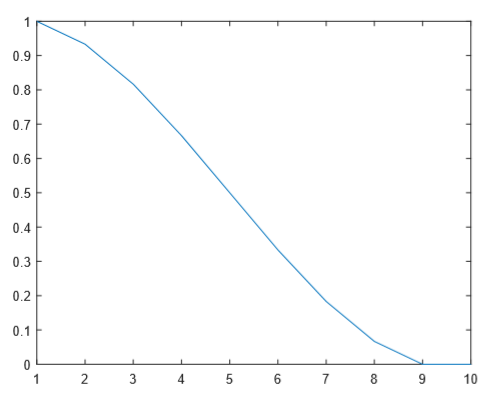
\includegraphics[scale=0.5]{p1}
\end{center}


\subsection*{Part d}
We can use the expression found in part d to come up with an expression for the same situation
where 4 questions are selected instead of 3.

We first notice that our scenarios change, we now have 3 different scenarios to consider in order
to find the probability of passing the exam, that is knowing 2, 3 and 4 topics from the exam.

For knowing 4 out of 4 topics, we use the same expression, changing 3s into 4s:
$\begin{pmatrix} n \\ 4 \end{pmatrix}$.
When 3 out of 4 topics were studied, we take the number of permutations for
$\begin{pmatrix} n \\ 3 \end{pmatrix}$ and multiply that by $10 - n $ the same way we did before
such as to get the total permutations including the 4th topic that was not studied for.
The final case, when 2 topics out of 4 were studied, we use the same principle as the latter, we
take the amount of permutations possible within these 2 topics and multiply it by the number
of permutations possible with the remaning $ 10 - n $ topics. This leaves us with:
$\begin{pmatrix} 10 - n \\ 2 \end{pmatrix}\begin{pmatrix} n \\ 2 \end{pmatrix}$

We sum these 3 scenarios and divide by the total amount of permutations of 10 topics in a 4 questions
exam:
\begin{equation}
    \frac{\begin{pmatrix} 10 - n \\ 2 \end{pmatrix}\begin{pmatrix} n \\ 2 \end{pmatrix}
        + (10 - n)\begin{pmatrix} n \\ 3 \end{pmatrix} + \begin{pmatrix} n \\ 4 \end{pmatrix}}
    {\begin{pmatrix} 10 \\ 4 \end{pmatrix}}
\end{equation}

We then obtain the following graph using code from appendix b.
\begin{center}
    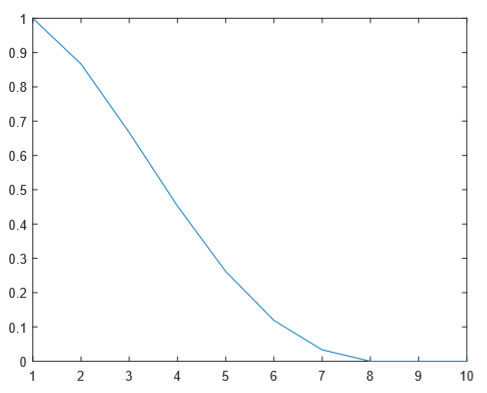
\includegraphics[scale=0.5]{p2}
\end{center}

Comparing this plot with the one from question c, we notice that for any equal amount
of topics studied, we have an overall higher change of passing with 4 topics in an exam
instead of 3. We also notice that the probability of passing becomes 1 at n = 8 instead of n = 9
for a an exam model containing 3 questions.

\subsection*{Part e}
The code for the stochastic simulation of the exam setup with three questions is
appended to this document in appendix c.
Please note that it is the function called \textbf{simulation3Questions} and that it
\textbf{may be used in the following questions}.


\subsection*{Part f}
The code for the extended simulation from part e, such that it runs the simulation
N times and returns the empirical mean is appended in appendix d.
Please note that it is the function called \textbf{simulationEmpiricalMean} and that it
\textbf{may be used in the following questions}.
Let's now compute the confidence intervals using the central limit theorem when
$ n = 7 $ with $ N = 1000 $ and $ N = 10000 $

We first need the mean and the variance thus we'll start by computing
$E[X_{i}]$ and $var(X_{i})$. We've seen in part c that an expression for
\begin{equation*}
    1 - E[X_{i}] = 1 - [ \frac{(10 - n) * \begin{pmatrix} n \\ 2 \end{pmatrix} + \begin{pmatrix} n \\ 3 \end{pmatrix}}{\begin{pmatrix} 10 \\ 3 \end{pmatrix}}]
    \leftrightarrow
    E[X_{i}] = [ \frac{(10 - n) * \begin{pmatrix} n \\ 2 \end{pmatrix} + \begin{pmatrix} n \\ 3 \end{pmatrix}}{\begin{pmatrix} 10 \\ 3 \end{pmatrix}}]
\end{equation*}
Thus, with $ n = 7$, $ E[X_{i}] = 0.8167 $.
To compute the variance, since the $ Y_{i} $ are independent,
\begin{equation}
    var(\frac{1}{n} \sum_{i=1}^N Y_{i}) = \frac{1}{n^2} \sum_{i=1}^N var(Y_{i}) = \frac{var(Y_{i})}{n} = \sigma^2
\end{equation}
Thus, using the empirical mean $ E[X_{i}] = 0.8167 $ and the equation for the variance in a bernouilli distributed
random variable: $ var(X) = \sqrt{p * (1 - p)} $, can get the standard deviation $\sigma$.
\begin{equation}
    \sigma = \sqrt{\frac{E[X_{i}] * (1 - E[X_{i})}{N}} = \sqrt{\frac{0.8167 * 0.1833‬}{N}} = \sqrt{\frac{0.3869}{N}}
\end{equation}
Here we have $N = 1000$ and $N = 10000$, thus:
TODO UPDATE THIS !!!!
$\sigma_{N=1000} = 0.01967 \\$
$\sigma_{N=10000} = \frac{0.3869}{10000} = 0.00622$

The 95\% confidence interval using the CLT is then
\begin{equation}
    [\mu − 2\sigma, \mu +2\sigma]_{N=1000} = [0.77736‬, 0.85604]_{N=1000}
\end{equation}
\begin{equation}
    [\mu − 2\sigma, \mu +2\sigma]_{N=10000} = [0.80426, 0.82914]_{N=10000}
\end{equation}


\subsection*{Part g}
TODO : USE CHEBYCHEV HERE FOR SIZE
The code for runing the simulation multiple times with both $N= 1000$ and $N= 10000$
is added to the appendix section f.
In theory, it is best to run the simulation with both Ns as many times as possible to
get the most accurate estimation. In practise though, running a simulation say 1000 or more
times when it already simulates N runs is not really feasible. I settled to run the $ N = 1000$
simulation 300 times as it seemed to be a manageable amount to handle by my computer and 
I ran it with $ N = 10000$ 100 times. Both of these values seemed to give me very similar
results at every run thus I assumed I ran the simulation enough times.

I've found that for running the simulation 300 times with $N = 1000$, about 82\% of empirical means
fall within the confidence interval. When running the simulation 100 times with $N = 10000$ 
the values are higher with 99\% of empirical means falling within the confidence interval.

This makes sense as the standard deviation when $N = 10000$ is much lower than when $N = 1000$,
we are also getting every empirical mean with $ N = 10000$ thus making the value much more likely to be
very similar at every run.

\subsection*{Part h}

In the case that subjects are more predictable if they came up in 
last years exam then, students
might change their studying strategy to, in general, study those topics more than other ones.
However other students might still decide to focus on other topics thus I have decided to use the same
weighing system for both drawing topics to study for a student and for the exam questions.
I have decided that giving a cumulated probability of 50\% to the 3 topics drawn last year and the final
50\% to the other 7 topics would be an interesting case to consider as that make 3 topics much likely
to be drawn but not too much so that only studying these 3 topics would guarantee a pass.
Using the code from appendix part g, I was able to obtain the plot prvided in appendix part h.
We notice that overall, for any value of studied topic n, more students will pass the exam
as they adapt to the topics drawn being more predictable.
Let's now consider the case where an exam that was drawn 
in the previous year is less likely to be drawn this year. Using the following weights: \\
$ w = [0.5/10 0.5/10 0.5/10 1.214/14 1.214/14 1.214/14 1.214/14 1.214/14 1.214/14 1.214/14];$ \\
I chose these by dividing the weight for drawn exams by 2 (thus going from $1/10$ to $0.5/10$) and
updating all 7 remaining topics weights accordingly.
We notice that overall, for an equal amount of topics n studied, students are less likely to pass,
this is due to the fact that when topics from the previous year are more likely to be drawn, 
it is easier for students to focus studying on these topics and thus they are more likely to pass.
The plot obtained from this scenario is provided in the appendix section I.

In the case that students use a studying strategy which assumes topics from previous year are more likely
to appear this year when in fact topics are drawn uniformly would mean that for the same number
of topics studied n, less students will pass due to the fact that more students will give priority to
studying 3 topics out of 10 (as their weight would be considered higher), when in fact all 10 topics
have the same, uniform, weighing. The plot obtained from this simulation is provided in the appendix section J.

\section*{Question 2}
Data id: $\#id:0.29:0.5-0.374:2-0.584:2-0$

\subsection*{Part a}

Discuss the 
strengths and weaknesses of using this approach to evaluate relative difficulty of the
questions

The plots for the PMF of all three questions are added to the appendix, respecively section K, L and M
for question 1, 2 and 3. The code used to obtain such plots is also provided in the appendix, section N.

Using question 3 as a baseline to assess the difficulty of an exam question, we clearly notice an interesting
phenomenon for the question 1. There is a very little, somewhat uniform proportion of students with
grades ranging from 0 to 95. For all of these grades we observe the probability for a student obtaining it 
to be less than $ 0.75 $. We also then notice a massive spike for the probability of obtaining a grade
of 100. This is very different from the expected student distribution and suggests that in this question
it is very easy to obtain a grade of 100 given that a student studied that topic. If not then students seem to 
gamble on their answers giving them a grade ranging from 0 to 95\%.

Question 2 seem to have a distribution similar to question 3 however, while question 3 seem to have a good proportion
of students with grades ranging between 10\% and 60\%, question 2 seem to have be ranging on the side of higher side of grades.
With most students falling between 35\% and 80\%. This suggests that it is an easier question to answer
no matter the level of studying done by a student on this topic.


One of the reasons I see this way of approach of evaluating the difficulty of an exam being good is due to 
the fact that if an entire class struggles with a particular exam, ie a lot of grades appear to be on the low,
then that exam is likely to be hard.
On the other hand, we can see false positives too, for instance if topics appear that students were not prepared for
we will naturaly see low grades even though the exam is not necesarily hard.

\subsection*{Part b}
I have added the code for this question to the appendix, section O. I decided to
use binning with a range of 10\% as it seemed to clean up the amount of obtains means and variances
thus making it easier to work with. Using brackets of 10\% also means that we keep some level of acuracy,
making the ranges too big (say 25 or 30\%) would simply not be as accurate.  

\subsection*{Part c}
The code for this section is the same as the previous, it is added in the appendix, section O, the
plot is also in the appendix section P.

For question 1, we notice that the means for all categories is always above 40 meaning that even students
who did poorly in question 1 probably scored close to 40\%.
What we notice too is that for students who scored between 60 and 100\% in the first question all seem to get
a similar mean for question 2 (of about 50\%). Thus we can also assume that even by knowing the material it is
difficult to get a very high grade.

We can say about question 2 that it is easy to obtain some marks (about 40\%) however it is quite hard
to obtain a grade above 50\%.

We notice that for question 2, the means seem to grow as expected. That is the higher a student scored
in the first question the higher he is expected to score in question 2. The error range seems to be fairly
low for the most part with the expection of the range 0-9\% which is to be expected as it is very
likely that this category possibly did not study the topic for question 1 but perhaps did question 2.

However we also notice that the mean for students who obtained a grade higher than 60\% all obtained
a very similar mean (close 50), and a fairly low error interval, meaning that question is very likely
to be hard to answer.


\subsection*{Part d}
e how you could use linear regression to predict the mark for a question given
the student mark for question one

mark for question one is the input
feature and the dataset is the training data

calculations from parts
(b) and (c) discuss whether the assumption in linear regression that the mean is a
linear function of the features is appropriate

If not, discuss how the features used
in the regression model might be modified to better fit the data

Discuss whether
the type of randomness assumed in linear regression is appropriate or not for exam
marks. 

\subsection*{Part e}

\begin{equation*}
    \prod_{i = 1}^N\frac{1}{\sigma\sqrt{2\pi}} e^{-\frac{(x - S_{i} - D_{j})^2}{2\sigma^2}}
    = (\sigma^{2}2\pi)^{-N/2}e^{-\frac{1}{2\sigma^2}\sum_{i = 1}^N(S_{i} - D_{j})^2}
\end{equation*}
\subsection*{Part f}


\section*{Appendix}
\subsection*{Section 0}
The code in the following sections may make use of the following function:
\textbf{customNChooseK}. It is a function which uses nchoosek when $ n >= k $.
If not then it will return 0. Matlab's default implementation of this situation is
to throw an error which is why I decided to write this helper function.
\begin{lstlisting}
function [m] = customNChooseK(n,k)
    if(n < k)
        m = 0;
    else
       m = nchoosek(n,k); 
    end
end
\end{lstlisting}

\subsection*{Section A - Question 1c}
\begin{lstlisting}
y1 = zeros([1 10]);
x1 = 1:10;
% Compute the probability for all values of n
for n = x1
    y1(n) = 1 - 
        (((10-n)*
        (customNChooseK(n,2))/customNChooseK(10,3)) +
        (customNChooseK(n,3)/customNChooseK(10,3)));
end
plot(x1, y1);
\end{lstlisting}

\subsection*{Section B - Question 1d}
\begin{lstlisting}
y1 = zeros([1 10]);
x1 = 1:10;
% Compute the probability for all values of n
for n = x1
    y1(n) = 1 - (((10-n)*
    (customNChooseK(n,3))/customNChooseK(10,4))+
    (customNChooseK(n,4)/customNChooseK(10,4)) + 
    (customNChooseK(10-n,2)*(customNChooseK(n,2)/
    customNChooseK(10,4))));
end
%plot(x1, y1);
\end{lstlisting}

\subsection*{Section C - Question 1d}
\begin{lstlisting}
y1 = zeros([1 10]);
x1 = 1:10;
% Compute the probability for all values of n
for n = x1
    y1(n) = 1 - (((10-n)*
    (customNChooseK(n,3))/customNChooseK(10,4))+
    (customNChooseK(n,4)/customNChooseK(10,4)) + 
    (customNChooseK(10-n,2)*(customNChooseK(n,2)/
    customNChooseK(10,4))));
end
%plot(x1, y1);
\end{lstlisting}

\subsection*{Section D - Question 1e}
\begin{lstlisting}
function [X] = simulation3Questions(n)
    % number of topics
    a=1:10;
    % questions drawn
    questions = randperm(numel(a),3);
    % draw for studied subjects
    studiedSubjects = randperm(numel(a),n); 
    
    % get common topics
    pos=intersect(questions, studiedSubjects);
    if(length(pos) >= 2)
        X = 1; 
    else 
        X =0;
    end
end    
\end{lstlisting}

\subsection*{Section E - Question 1f}
\begin{lstlisting}
function [X] = simulationEmpiricalMean(n, N)
    passCount = 0;
    for i = 1:N
        % number of topics
        a=1:10;
        % questions drawn
        questions = randperm(numel(a),3);
        % draw for studied subjects
        studiedSubjects = randperm(numel(a),n); 

        % get common topics
        pos=intersect(questions, studiedSubjects);
        if(length(pos) >= 2)
            passCount = passCount + 1;
        end 
    end
    
    X = passCount / N;
end  
\end{lstlisting}

\subsection*{Section F - Question 1g}
\begin{lstlisting}
count = 0;
% 1000 or 10000 depending on simulation to run
N = 10000;
% Amount of times to run simulation
size = 100;
% Values of the confidence interval (here for N = 10000)
lo = 0.80426;
hi = 0.82914;

% Run simulation size times and increment count if 
% the mean falls within the CI
for i = 1:size
    % function from appendix section f
    % returns the empirical mean.
    simMean = simulationEmpiricalMean(7, N);
    if(simMean >= lo && simMean <= hi)
        count = count + 1;
    end
end
% Display % of means falling within confidence interval
disp(count/size * 100);
\end{lstlisting}

\subsection*{Sectiong G - Question 1h}
\begin{lstlisting}
% run simulation for all values of n (topics studied)
y1 = zeros([1 10]);
x1 = 1:10;
N = 10000;
% Compute the probability for all values of n
for n = x1
    y1(n) = simulationEmpiricalMeanWeighted(n, N);
end
plot(x1, y1);

function [X] = simulationEmpiricalMeanWeighted(n, N)
    passCount = 0;
    % weighs for drawing topics
    w = [1/6 1/6 1/6 1/14 1/14 1/14 1/14 1/14 1/14 1/14];
    % number of topics
    topics=1:10;
    for i = 1:N
        % questions drawn using weights
        questions = datasample
            (topics,3,'Weights', w,'Replace',false);
        % topics studied drawn using weights
        studiedSubjects = datasample
            (topics,n,'Weights', w,'Replace',false);
        % get common topics
        inters=intersect(questions, studiedSubjects);
        if(length(inters) >= 2)
            passCount = passCount + 1;
        end 
    end
    
    X = passCount / N;
end 
\end{lstlisting}

\subsection*{Section H - Question 1h}
Scenario where topics drawn in a previous exam is more likely
to appear this year, and students adapt their studying accordingly.\\
y axis: Empirical mean of a student passing with N = 10000 \\
x axis: Number n of subjects studied by students
\begin{center}
    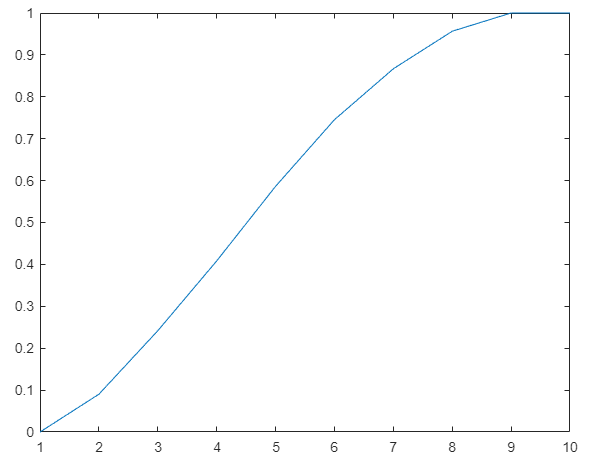
\includegraphics[scale=0.5]{p3}
\end{center}

\subsection*{Section I - Question 1h}
Scenario where a topic drawn in a previous exam 
is less likely to appear this year. Using weights:\\
$ w = [0.5/10 0.5/10 0.5/10 1.214/14 1.214/14 1.214/14 1.214/14 1.214/14 1.214/14 1.214/14];$\\
y axis: Empirical mean of a student passing with N = 10000 \\
x axis: Number n of subjects studied by students
\begin{center}
    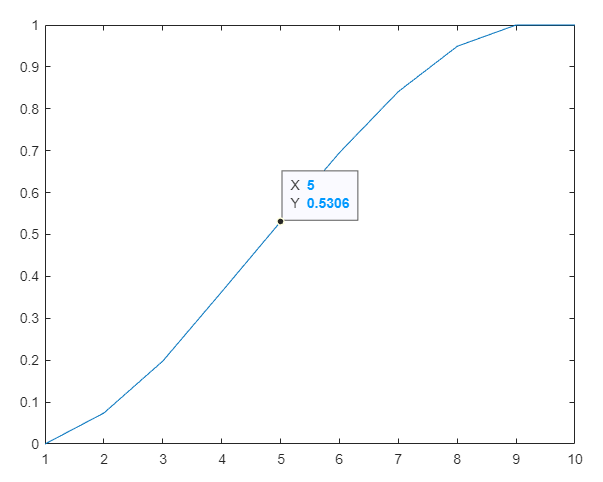
\includegraphics[scale=0.5]{p4}
\end{center}

\subsection*{Section J - Question 1h}
Scenario where student assume that a topic drawn in a previous exam is more likely
to appear this year, when they are actually drawn uniformly.\\
y axis: Empirical mean of a student passing with N = 10000 \\
x axis: Number n of subjects studied by students
\begin{center}
    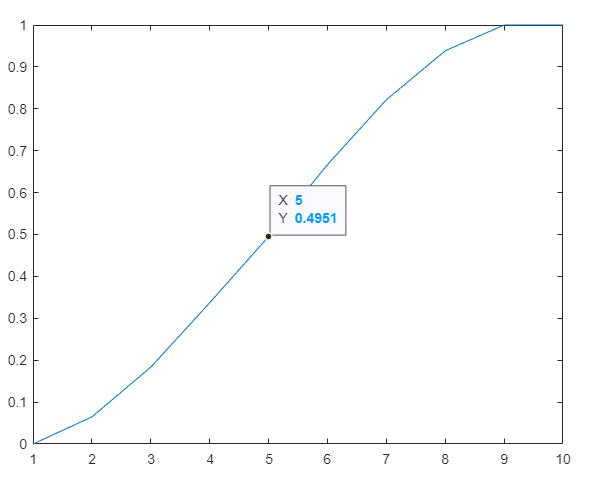
\includegraphics[scale=0.5]{p5}
\end{center}

\subsection*{Section K - Question 2a}
Scenario where student assume that a topic drawn in a previous exam is more likely
to appear this year, when they are actually drawn uniformly.\\
y axis: Empirical mean of a student passing with N = 10000 \\
x axis: Number n of subjects studied by students
\begin{center}
    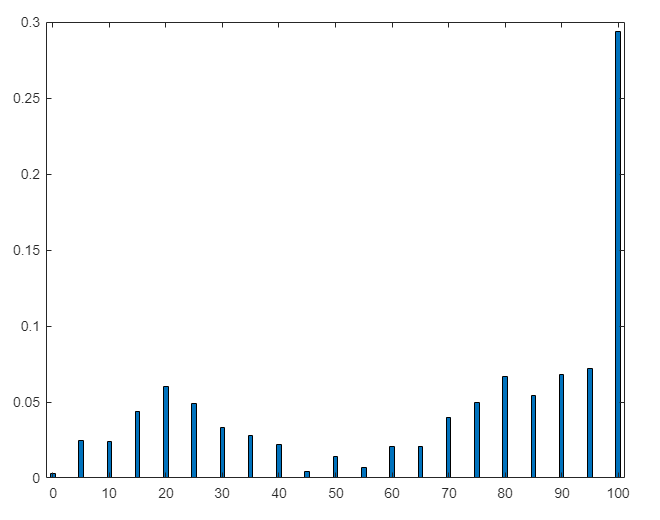
\includegraphics[scale=0.5]{q2_a}
\end{center}

\subsection*{Section L - Question 2a}
Scenario where student assume that a topic drawn in a previous exam is more likely
to appear this year, when they are actually drawn uniformly.\\
y axis: Empirical mean of a student passing with N = 10000 \\
x axis: Number n of subjects studied by students
\begin{center}
    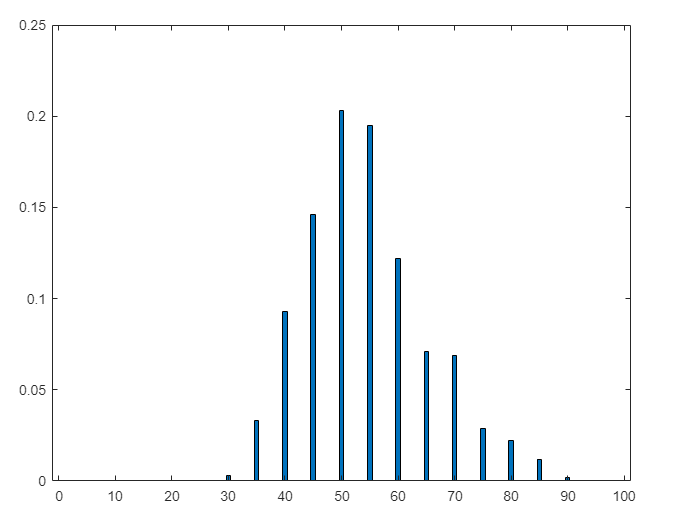
\includegraphics[scale=0.5]{q2_b}
\end{center}

\subsection*{Section M - Question 2a}
Scenario where student assume that a topic drawn in a previous exam is more likely
to appear this year, when they are actually drawn uniformly.\\
y axis: Empirical mean of a student passing with N = 10000 \\
x axis: Number n of subjects studied by students
\begin{center}
    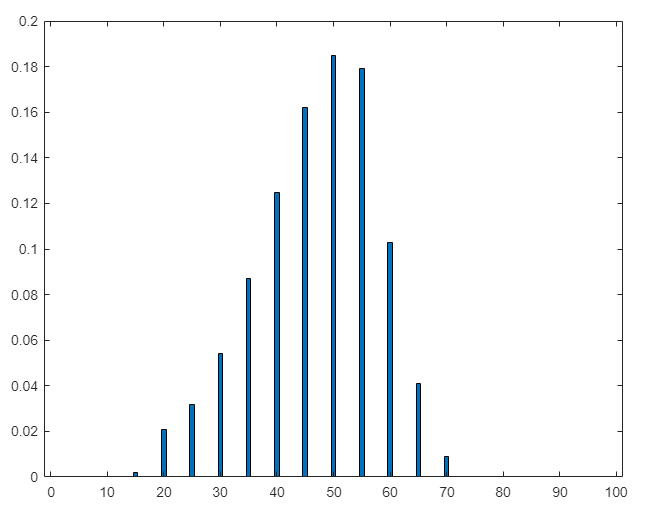
\includegraphics[scale=0.5]{q2_c}
\end{center}


\subsection*{Section N - Question 2a}
Code used to obtain the above 3 plots.\\
\begin{lstlisting}
data = load('data.txt');
nstudents = length(data(:,1));

countsQ1=zeros(1, 101);
countsQ2=zeros(1, 101);
countsQ3=zeros(1, 101);

gradesQ1 = data(:,1);
gradesQ2 = data(:,2);
gradesQ3 = data(:,3);


for i=1:nstudents
    countsQ1(gradesQ1(i) + 1) = 
        countsQ1(gradesQ1(i)+ 1) + 1; 
    countsQ2(gradesQ2(i) + 1) = 
        countsQ2(gradesQ2(i)+ 1) + 1; 
    countsQ3(gradesQ3(i) + 1) = 
        countsQ3(gradesQ3(i)+ 1) + 1; 
end
% Plot the graph
events = 0:100;
bar(events, countsQ1/nstudents);
bar(events, countsQ2/nstudents);
bar(events, countsQ3/nstudents);
\end{lstlisting}

\subsection*{Section O - Question 2b and 2b}
\begin{lstlisting}
% Q2 b
data = load('data.txt');
m = 1000;
averages = zeros([10,1]);
vars = zeros([10,1]);
intervals=[];

for i = 1:10
    c=1;
    firstQuestionStudents = zeros([1,1]);
    
    for j = 1:m
        if (data(j, 1) < i*10) && 
            (data(j, 1) >= (i*10)-10)
            firstQuestionStudents(c) = j;
            c = c + 1;
        end
    end
      
    [fm,fn] = size(firstQuestionStudents);
    tempV = [];
    
    for zq = 2:3
        mean = 0;
        for zs = 1:fn        
            tempV = [tempV; 
                data(firstQuestionStudents(zs),zq)];
            mean = mean + 
                data(firstQuestionStudents(zs),zq);
        end
        
        vars(i,zq-1) = var(tempV);
        averages(i,zq-1) = mean/fn;
        
        %Q2 c
        se = sqrt(vars(i,zq-1))/sqrt(fn);
        intervals(i,zq-1,1) = averages(i)-(2*se);
        intervals(i,zq-1,2) = averages(i)+(2*se);
    end 
end
figure
hold on
xAxis = 10:10:100;
yAxis = [reshape(averages(:,1),1,10);
    reshape(averages(:,2),1,10)];
bar(xAxis, yAxis);

err = ones([10,1]);
for i = 1:10
    err(i) = intervals(i,1,2) - intervals(i,1,1);
end
errorbar(xAxis-1.25,reshape(averages(:,1),1,10), err);

err = ones([10,1]);
for i = 1:10
    err(i) = intervals(i,2,2) - intervals(i,2,1);
end
errorbar(xAxis+1.25,reshape(averages(:,2),1,10), err);
\end{lstlisting}

\subsection*{Section P - Question 2c}
x axis: Grade obtained by students in question 1. \\
y axis: Mean for question 2 and 3. \\
Blue bars: values for question 2. \\
Red bars: values for question 3.
\begin{center}
    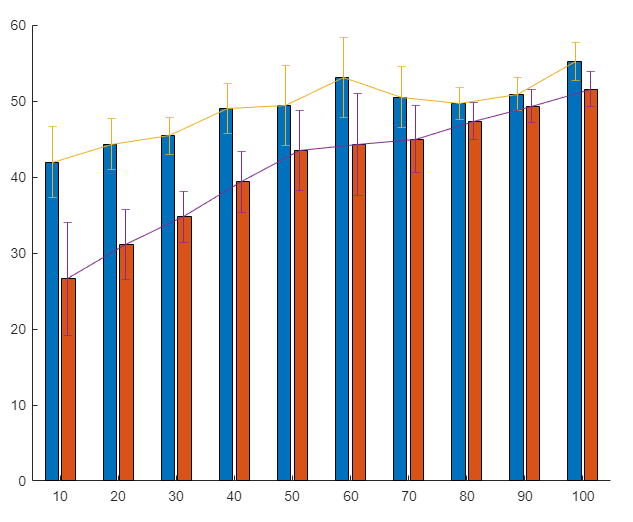
\includegraphics[scale=0.5]{q2_d}
\end{center}


\end{document}